% !TEX root = ../../document.tex

\documentclass{subfiles}

\begin{document}

  \chapter{Algoritmo PageRank}
  \label{chap:pagerank}

    \section{Introducción}
    \label{sec:pagerank_intro}

      \paragraph{}
      El algoritmo \emph{PageRank} fue nombrado por primera vez en el trabajo \emph{The PageRank citation ranking: Bringing order to the web} \cite{page1999pagerank} publicado por \emph{Larry Page} y \emph{Sergey Brin}. La motivación del mismo fue tratar de realizar un \emph{ranking de importancia} (o relevancia) sobre los nodos de un \emph{grafo dirigido no ponderado} de tal manera que este esté basado únicamente en la estructura de dicho grafo.

      \paragraph{}
      La motivación de dicho trabajo fue la de tratar de mejorar el ranking de resultados del buscador de sitios web \emph{Google} en que estaban trabajando. Hasta la publicación de dicho trabajo, los sistemas de búsqueda se basaban en heurísticas como el número de ocurrencias de la palabra clave sobre la cual se basaba la búsqueda o el número de enlaces hacia dicha página.

      \paragraph{}
      Sin embargo, los rankings basados en este tipo de estrategias podían ser fácilmente manipulables con el fin de tratar de conseguir posicionarse en las primeras posiciones del sistema de búsqueda. Por ejemplo, una página web que se basara en la repetición de la misma palabra muchas veces, entonces aparecería en primer lugar en rankings basados en el número de ocurrencias para dicha palabra clave. En el caso de rankings basados en el número de enlaces hacia dicha página, tampoco sería complejo manipular el resultado creando un número elevado de páginas web que contuvieran links hacia la página para la cual se pretende mejorar su posicionamiento.

      \paragraph{}
      La solución propuesta por \emph{Page} y \emph{Brin} para tratar de solucionar dicha problemática se basa en la generación de un ranking sobre los sitios web basado en la estructura del grafo subyacente, de tal manera que los vértices (sitios web) sobre los cuales existan aristas (enlaces) que provengan de otros vértices relevantes, tendrán una puntuación mayor que la de vértices que cuyo sub-conjunto de aristas los relacione con otros vértices menos relevantes.

      \paragraph{}
      La idea en que se basa el ranking se refiere por tanto a que los sitios web a los cuales se puede acceder a partir de otros sitios web considerados como importantes, entonces deberán encontrarse en primeras posiciones. Esta idea se extiende de manera inductiva sobre todos los vértices del grafo, puesto que tal y como veremos en las siguientes secciones converge hacia un estado estable (o \emph{distribución estacionaria} desde el punto de vista estadístico)

      \paragraph{}
      Para tratar de facilitar la comprensión acerca de esta idea a continuación se expone un ejemplo: Supongamos que en una red social como \emph{Twitter} (la cual se puede entender como un conjunto de usuarios que se relacionan entre si mediante relaciones de seguimiento, por lo que se puede ver como un grafo dirigido no ponderado donde el conjunto de usuarios se refiere a los vértices y el conjunto de relaciones de seguimiento con las aristas) un usuario habitual (el cual no tiene un número elevado de seguidores) comienza a seguir a un antiguo amigo de la universidad, el cual tampoco tiene un gran número de seguidores.

      \paragraph{}
      La red social \emph{Twitter} envía una notificación a todos seguidores del usuario indicando que este ha empezado a seguir a su amigo de la universidad. Puesto que su número de seguidores es bajo dicha acción no tendrá una gran relevancia y muy probablemente nadie más comience a seguir al amigo de la universidad. Sin embargo, supongamos que nuestro usuario, en lugar de tener un conjunto reducido de seguidores, es una persona influyente en la red social, a la cual siguen millones de personas, entonces la notificación del nuevo seguimiento le llegará a muchos más usuarios y probablemente el amigo de la universidad verá como su número de seguidores aumenta notablemente.

      \paragraph{}
      A grandes rasgos, esta es la idea en que se basa el algoritmo \emph{PageRank}, es decir, la puntuación de un vértice del grafo se basa en la relevancia de los vértices que contienen aristas que apuntan hacia el propio vértice.

      \paragraph{}
      La idea inicial del algoritmo \emph{PageRank} era la de realizar un ranking basado en la estructura del grafo de la web (\emph{Web Graph}), sin embargo, tal y como se verá a lo largo del capítulo, los conceptos matemáticos en que se basa dicho ranking son extrapolables a cualquier entorno que se pueda representar a partir de una red o grafo. En el trabajo \emph{PageRank beyond the Web}\cite{gleich2015pagerank} \emph{Gleich} realiza un estudio acerca de los distintos entornos sobre los cuales se han aplicado estas ideas.

      \paragraph{}
      Entre otros, se han realizado trabajos sobre los cuales se ha aplicado el algoritmo \emph{PageRank} en áreas tan dispares como la Biología, para analizar las células más importantes a partir de las interrelaciones entre ellas. También se ha aplicado en el sector de la neurociencia por razones similares. En el caso de la literatura, se ha aplicado sobre el grafo generado a partir del sistema de citaciones de artículos de investigación. Otros ámbitos de aplicación han sido sistemas de planificación de tareas o incluso estudios acerca de resultados en deportes, para conocer los encuentros más relevantes.


      \paragraph{}
      El resto del capítulo se organiza como sigue: Lo primero será hablar de \emph{Paseos Aleatorios} en la sección \ref{sec:random_walks}, lo cual permitirá comprender en mayor medida las idea sobre las cuales se basa el ranking \emph{PageRank}. A continuación se realizará una definición formal acerca del problema y lo que se pretende resolver en la sección \ref{sec:pagerank_formal_definition}. Una vez entendido el problema sobre el que se está tratando, en la sección \ref{sec:pagerank_algorithm} se describen las formulaciones para resolver el problema desde un punto de vista \emph{Algebraico} (sección \ref{sec:pagerank_algorithm_algebraic}), \emph{Iterativo} (sección \ref{sec:pagerank_algorithm_iterative}) y \emph{basado en Paseos Aleatorios} (sección \ref{sec:pagerank_algorithm_random_walks}). El siguiente paso es discutir cómo se puede añadir personalización al ranking, lo cual se lleva a cabo en la sección \ref{sec:pagerank_algorithm_personalized}. Por último, se presentan distintas alternativas al algoritmo \emph{PageRank} en la sección \ref{sec:pagerank_alternativas}, en la cual se habla de \emph{HITS} (sección \ref{sec:hits}), \emph{SALSA} (sección \ref{sec:salsa}) y \emph{SimRank} (sección \ref{sec:simrank}). Finalmente se realiza un breve resumen del capítulo en la sección \ref{sec:pagerank_conclusions}.


    \section{Paseos Aleatorios}
    \label{sec:random_walks}

      \paragraph{}
      En esta sección se trata el concepto de \emph{Paseos Aleatorios}, el cual está íntimamente relacionado con el algoritmo \emph{PageRank}. Para el desarrollo de esta sección se ha utilizado como herramienta bibliográfica el libro \emph{Randomized algorithms} \cite{motwani2010randomized} de \emph{Motwani} y \emph{Raghavan}, concretamente se ha prestado especial atención al \emph{capítulo 6: Markov Chains and Random Walks}. El resto de la sección se basará en la descripción de propiedades relacionadas con \emph{Paseos Aleatorios} para finalizar ilustrando la relacion de estos con \emph{PageRank}

      \paragraph{}
      Lo primero que haremos será describir en qué consiste un \emph{Paseo Aleatorio}. Para ello nos referiremos al grafo $G=(V,E)$ dirigido y no ponderado, el cual esta compuesto por $n = card(V)$ vértices y $m=card(E)$ aristas. Un paseo aleatorio se refiere entonces a un camino de longitud $l$ con origen en el vértice $v_{i_1}$ y final en $v_{i_l}$. Para que dicho camino constituya un paseo aleatorio, cada paso debe haber sido generado seleccionando de manera uniforme el siguiente vértice a visitar de entre los adyacentes al vértice actual. Nótese que este comportamiento puede ser visto como el promedio del modo en que los usuarios navegan por internet, de tal manera que acceden a páginas web mediante los enlaces que encuentran en la página que están visualizando. A continuación se describen las \emph{Cadenas de Markov} por su relación como herramienta de estudio para los paseos aleatorios.


      \subsection{Cadenas de Markov}
      \label{sec:markov_chains}

        \paragraph{}
        Para el estudio de paseos aleatorios, es apropiado utilizar la abstracción conocida como \emph{Cadenas de Markov}, las cuales están íntimamente relacionadas con el concepto de grafo y máquina de estados. Una \emph{Cadena de Markov} $M$ se define como un proceso estocástico que consta de $n$ posibles estados, los cuales tienen asociadas un conjunto de probabilidades denotadas como $p_{ij}=\frac{A_{ij}}{d^-(i)}$ para indicar la probabilidad con la cual se pasará del estado $i$ al estado $j$.

        \paragraph{}
        Dichas probabilidades se pueden representar de manera matricial sobre una matriz de transiciones $P$ de tamaño $n*n$, de tal manera que la posición $(i,j)$ contenga el valor $p_{ij}$ construido tal y como se indica en el párrafo anterior. Notese por tanto, que $\sum_{j}p_{ij}=1$ para que la distribución de probabilidades sea válida, es decir, la suma de probabilidades para las transiciones sobre cada estado deben sumar $1$.

        \paragraph{}
        Supóngase que se realiza un paseo aleatorio sobre la \emph{Cadena de Markov} $M$ cuya longitud $l$ es muy elevada ($l \gg n^2$), entonces, es fácil intuir que se visitará más de una vez cada estado. Sin embargo, el ratio de veces que se visitará cada estado muy probablemente no se distribuirá de manera uniforme, sino que habrá estados que serán visitados muchas más veces que otros. Esto depende en gran medida de la matriz de transiciones $P$. A la distribución de probabilidad generada sobre el ratio de visitas sobre cada nodo tras aplicar un paseo aleatorio de longitud elevada se le conoce como \emph{distribución estacionaria} y se denota como $\pi$.

        \begin{figure}
          \centering
          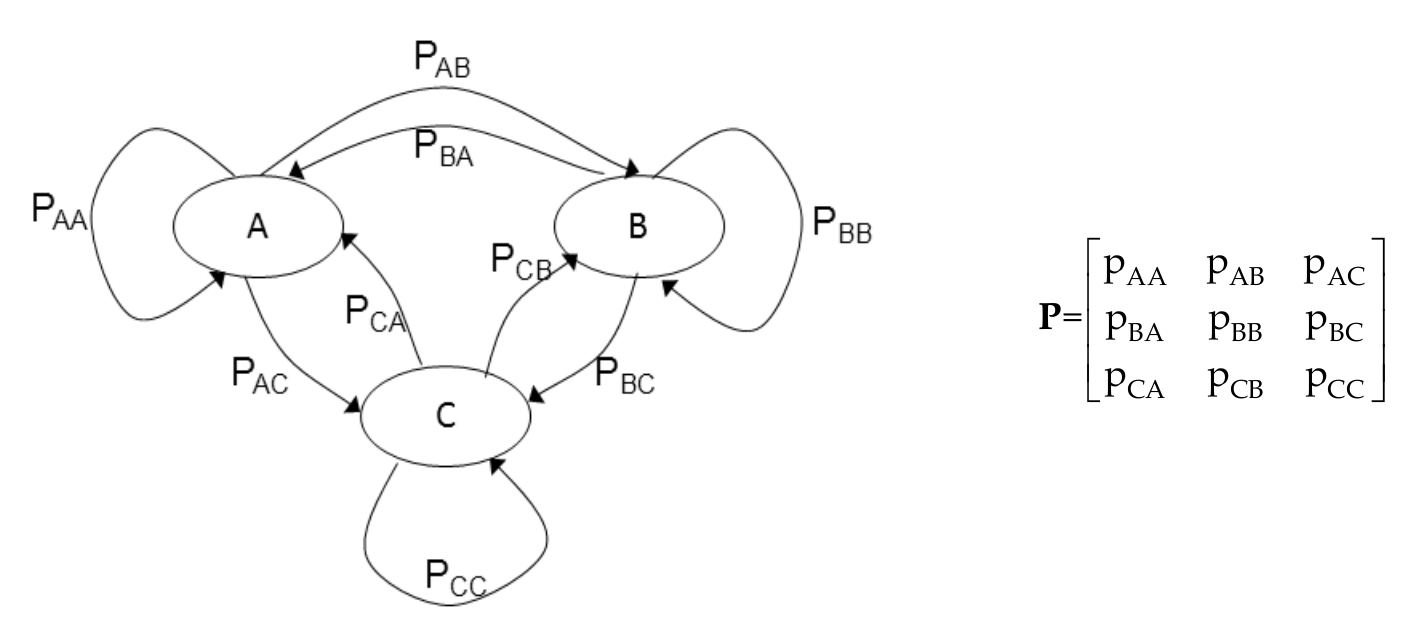
\includegraphics[width=0.6\textwidth]{markov-chain-example}
          \caption{Ejemplo de \emph{Cadena de Markov}. (Extraído de \cite{sanchez2012wireless})}
          \label{img:markov_chain_example}
        \end{figure}

        \paragraph{}
        En la figura \ref{img:markov_chain_example} (Extraído de \cite{sanchez2012wireless}) se muestra una cadena de Markov constituida por 3 estados, tanto en su forma de grafo dirigido como de forma matricial.

        \paragraph{}
        La distribución estacionaria $\pi$ existe siempre que la \emph{Cadena de Markov} $M$ permita que a partir de un determinado estado $i$, se pueda llegar al menos a otro estado $j$. La razón se debe a que si se llega al estado $i$ y este no contiene más posibles estados de salida, entonces el resto de épocas se seguirá en el mismo estado. A los estados que poseen esta característica se los denomina sumideros. La segunda restricción para que se pueda calcular la distribución estacionaria $\pi$ es que la matriz de transiciones $P$ no debe ser periódica, es decir, no debe contener ciclos de probabilidad constante sobre los cuales el paseo aleatorio se quedaría iterando de manera indefinida.

        \paragraph{}
        Las definiciones descritas en este apartado se pueden extender de manera trivial al caso de grafos dirigidos sin más que utilizar cada vértice del grafo como un estado y construir la matriz $P$ de tal manera que $p_{ij}=\frac{A_{ij}}{d^-(i)}$ donde $d^-(i)$ representa el cardinal de aristas cuyo origen es el vértice $i$. Tal y como se verá posteriormente, el vector $\pi$ se corresponde con el resultado obtenido por el algoritmo \emph{PageRank} sobre una matriz $P$ de transiciones modificada.

      \subsection{Matriz Laplaciana de Paseos Aleatorios Normalizada}
      \label{sec:random_walk_normalized_laplacian_matrix}

        \paragraph{}
        En la sección \ref{sec:laplacian_matrix} se habló sobre la \emph{Matriz Laplacina}, la cual es una estrategia de representación, que ilustra distintas propiedades sobre el grafo subyacente. En este caso se describe una variación de la misma que es más apropiada para problemas relacionados con \emph{Paseos Aleatorios}. Esta se denota como $L^{{{\text{rw}}}}$ y se denomina \emph{Matriz Laplaciana de Paseos Aleatorios Normalizada}. La estrategia de construcción de la misma se indica en la ecuación \eqref{eq:random_walk_normalized_laplacian_matrix}. Esto consiste en asignar a la posición $(i,j)$ el opuesto de la probabilidad de transición del vértice $i$ al vértice $j$. Además, en la diagonal $(i,i)$ se asigna el valor $1$ cuando el grado del vértice es mayor que $0$.

        \begin{equation}
        \label{eq:random_walk_normalized_laplacian_matrix}
          L_{{i,j}}^{{{\text{rw}}}}:={
          \begin{cases}
            1&{\mbox{if}}\ i=j\ {\mbox{and}}\ d(v_{i})\neq 0\\
            -{P_{ij}}&{\mbox{if}}\ i\neq j\ {\mbox{and}}\ v_{i}{\mbox{ is adjacent to }}v_{j}\\
            0&{\mbox{otherwise}}.
          \end{cases}}
        \end{equation}


      \paragraph{}
      Una vez descritos los \emph{Paseos Aleatorios}, junto con las \emph{Cadenas de Markov} y la \emph{Matriz Laplaciana de Paseos Aleatorios Normalizada}, ya se está en condiciones suficientes como para describir de manera formal el \emph{PageRank} de un determinado grafo, que se realizará en la siguiente sección. Para ello, se indicarán las dificultades que surgen sobre este problema en grafos reales, así como las soluciones utilizadas para poder hacer frente a estas.

    \section{Definición Formal}
    \label{sec:pagerank_formal_definition}

      \paragraph{}
      Se define el \emph{PageRank} como la \emph{distribución estacionaria} $\pi$ de un determinado grafo dirigido no ponderado $G$ sobre el cual, la matriz de transiciones $P$, ha sido ligeramente modificada. Tal y como se ha visto en la sección anterior, la \emph{distribución estacionaria} consiste en la probabilidad de encontrarse en el estado $i$ durante un paseo aleatorio de longitud elevada sobre la \emph{Cadena de Markov} $M$. Tal y como se ha indicado, para que una cadena de Markov sea válida, entonces no deben existir estados \emph{sumideros} (no tienen posibles estados próximos).

      \paragraph{}
      Por estas razones, obtener la \emph{distribución estacionaria} de un grafo $G$, este no debe contener vértices \emph{sumideros}. La solución que proponen \emph{Page} y \emph{Brin} en \cite{page1999pagerank} para encontrar la \emph{distribución estacionaria} o \emph{PageRank} del grafo generado por los enlaces de la web (\emph{Web Graph}) es añadir un determinado índice de probabilidad sobre el cual los usuarios dejan de seguir los enlaces entre páginas web para acceder a otra distinta introduciendo la URL directamente. El apoyo en esta estrategia soluciona por tanto el problema de los vértices \emph{sumidero}, además de asemejarse en un mayor grado al comportamiento real de un usuario que navega por internet.

      \paragraph{}
      En \cite{page1999pagerank} \emph{Page} y \emph{Brin} proponen la modificación de la matriz de transiciones $P$ para la adaptación descrita en el párrafo superior, la cual se indica en la ecuación \eqref{eq:pagerank_transition_matrix}. De esta manera, se representa la situación en la cual un determinado usuario que llega a una página web sin enlaces hacia otras (\emph{sumidero}), accede a otra seleccionada de manera uniforme (esto se modeliza mediante el vector $p$ construido de tal manera que  $p_{i} = \frac{1}{n}, \ \forall i \in [1,n]$). Además, se añade un determinado índice $\beta$, que se corresponde con la probabilidad de que el usuario continúe seleccionando enlaces en la página actual o ,por contra, acceda a otra selecionandola de manera uniforme. Típicamente el valor $\beta$ se fija a $0.85$, sin embargo, admite cualquier valor contenido en el intervalo $[0,1]$.

      \begin{equation}
      \label{eq:pagerank_transition_matrix}
        p'_{ij} =
        \begin{cases}
          \beta * \frac{A_{ij}}{d^-(i)} + (1- \beta) * p_{i} & \mbox{if} \ d^-(i) \neq 0 \\
          p_{i}&\mbox{otherwise}
        \end{cases}
      \end{equation}

      \paragraph{}
      Tal y como se ha indicado anteriormente, el vector $p$ representa la distribución de probabilidad referida a los saltos que un usuario lleva a cabo entre sitios web sin tener en cuenta los enlaces del sitio web actual. En el párrafo anterior se ha indicado que este vector es construido siguiendo una distribución uniforme, por tanto, esto puede ser visto de tal manera que la probabilidad de saltar de un sitio web a otro es la misma. Sin embargo, dicha acción podría seguir una distribución de probabilidad distinta dependiendo de cada usuario de la red. Por tanto, en \cite{page1999pagerank} se habla de \emph{PageRank Personalizado} cuando el vector $p$ sigue una distribución de probabilidad distinta de la uniforme (desviada hacia los sitios web a los que más accede el usuario).

      \paragraph{}
      En el trabajo \emph{Topic-sensitive pagerank} \cite{haveliwala2002topic} \emph{Haveliwala} propone la generación de 16 \emph{distribuciones estacionarias} (\emph{PageRanks}) distintas mediante la personalización del vector $v$, para después realizar una combinación de estas y así conseguir que el ranking final sea personalizado.

      \paragraph{}
      Una vez descritas las transformaciones necesarias a realizar sobre la matriz de transiciones $P$ para que esta se adapte a la estructura de grafos con vértices \emph{sumidero}, y que además emule de manera más apropiada el comportamiento de un determinado usuario sobre el grafo de la web (\emph{Web Graph}), lo siguiente es explicar cómo se puede obtener la \emph{distribución estacionaria} o \emph{PageRank} del grafo. Para ello, a continuación se describe el \emph{Teorema de Perron–Frobenius}, que aporta una idea acerca de la manera en que se calcula, además de asegurar la convergencia de la matriz de transiciones hacia un estado estacionario del vector $\pi$.

      \subsection{Teorema de Perron–Frobenius}
      \label{sec:perron_frobenius_theorem}

        \paragraph{}
        El \emph{teorema de Perron–Frobenius} se refiere a la existencia de un \textbf{único} \emph{vector propio} (\emph{eigenvector}) para las matrices cuadradas reales positivas. Dicha descripción ha sido extraída del documento \emph{Notes on the perron-frobenius theory of nonnegative matrices} \cite{boyle2005notes} de \emph{Boyle} (profesor de matemáticas de la \emph{Universidad de Marylan}). En primer lugar es necesario describir los conceptos de \emph{vector propio} como de \emph{matriz cuadrada real positiva} para después ver que la \emph{distribución estacionaria} y la \emph{matriz de transiciones} referidos a una \emph{Cadena de Markov} $M$ pueden ser vistos de esta manera.

        \paragraph{}
        Una \emph{matriz cuadrada real positiva} $A$ es aquella formada por $n$ filas y $n$ columnas ($n*n$ celdas) para las cuales $\forall i,j \in [1,n]$ se cumple que $A_{ij} \in \mathbb{R} \geq 0$. Tal y como se puede apreciar, la \emph{matriz de transiciones modificada} $P'$ del grafo $G$ cumple esta propiedad ya que $\forall i,j \in [1,n] \ P'_{ij} \in [0,1]$.

        \paragraph{}
        En cuanto al concepto de \emph{vector propio} $\lambda$ de un matriz, se refiere a un vector de $n$ columnas ($1*n$) tal que cuando es multiplado por una determinada matriz $A$, el resultado sigue siendo el mismo. Es decir, se cumple que $\lambda = \lambda * A$. Notese por tanto, que esta idea es equivalente a la \emph{distribución estacionaria} desde el punto de vista de llegar a un estado estable.

        \paragraph{}
        El teorema de \emph{teorema de Perron–Frobenius} asegura por tanto, que para una \emph{matriz cuadrada real positiva} $A$ tan solo existe un único \emph{vector propio} $\lambda$ y el conjunto de valores de este se es estrictamente positivo, es decir, $\forall i \in [1,n] \ \lambda_i \geq 0$. La demostración de dicho teorema puede encontrarse en \cite{boyle2005notes}.

        \paragraph{}
        Además, en el caso de que la matriz $A$ haya sido normalizada por columna, es decir, se cumpla que $\forall i \in [1,n] \ \sum_j A_{ij} = 1$, entonces el autovector $\lambda$ también seguirá la propiedad de normalización ($\sum_i \lambda_i = 1$). Gracias a este resultado es posible calcular la \emph{distribución estacionaria} $\pi$ de una \emph{Cadena de Markov} como el \emph{vector propio} de su matriz de transiciones.

      \paragraph{}
      Una vez descrito el \emph{teorema de Perron–Frobenius} ya se está en condiciones suficientes para describir las distintas alternativas para calcular el \emph{PageRank} de un determinado grafo, el cual se calcula tal y como se ha indicado en esta sección, encontrando el \emph{vector propio} de la matriz de transición modificada de la cadena de Markov. Las distintas estrategias para obtener este resultado se describen en la siguiente sección.

    \section{Algoritmo Básico}
    \label{sec:pagerank_algorithm}

      \paragraph{}
      En esta sección se describe el método para obtener el vector \emph{PageRank} sobre un determinado grafo $G$. Para ello, es necesario fijar 3 parámetros los cuales se indican a continuación:
      \begin{itemize}
        \item Matriz de adyacencia $A$, que a partir de la cual se obtiene la estructura del grafo (Se habló de ella en la sección \ref{sec:adjacency_matrix}).
        \item El valor de probabilidad $\beta$ de seguir el paseo aleatorio a partir de la distribución del vértice actual (el cual se comentó en la sección anterior).
        \item El vector de personalización $p$ referido a la distribución de probabilidad de los saltos aleatorios entre vértices (también se habló en la sección anterior).
      \end{itemize}

      \paragraph{}
      Para calcular el \emph{vector propio} $\lambda$ existen distintas estrategias matemáticas. En esta sección se habla de dos estrategias, la primera de ellas basada en la resolución de un sistema de ecuaciones lineales mientras que la segunda se basa en acercamiento a la solución de manera iterativa. Tal y como se verá a continuación, la estrategia algebraica conlleva un coste computacional muy elevado, por lo que no es admisible sobre grafos de tamaño masivo. En estos casos se utiliza la estrategia iterativa u otras alternativas basadas en la generación de \emph{Paseos Aleatorios}.


      \subsection{Estrategia Algebraica}
      \label{sec:pagerank_algorithm_algebraic}

        \paragraph{}
        La idea de la estrategia algebraica se refiere a la búsqueda del vector $\lambda$ que resuelva la ecuación $\lambda = \lambda * P'$ como un sistema de ecuaciones lineales. Esto se puede llevar a cabo siguiendo el desarrollo de la ecuación \eqref{eq:pagerank_algorithm_algebraic_1}. Nótese que para ello no se utiliza la \emph{matriz de transiciones modificada} $P'$ explícitamente. En su lugar, esta es representada implícitamente a partir de las operaciones de \eqref{eq:pagerank_algorithm_algebraic_2} y \eqref{eq:pagerank_algorithm_algebraic_3}.

        \paragraph{}
        Para entender estas ecuaciones, lo primero es indicar la notación que se ha utilizado así como la interpretación de algunas operaciones: El símbolo $\boldsymbol{I}$ representa la matriz identidad ($1$'s en la diagonal y $0$'s en el resto) de tamaño $n$. El símbolo $d^-$ representa un vector columna de tamaño $n$ que representa en su posición $j$ el cardinal de aristas cuyo origen es el vértice $j$. Esto puede ser visto de la siguiente manera: $\forall j \in [1,n] \ \sum_i A_{ij} = d^{-}_{j}$. A nivel de operaciones es necesario resaltar el caso de la división $\frac{A}{d^-}$ por su carácter matricial. Esta se lleva a cabo realizando la división elemento a elemento por columnas.

        \begin{align}
          \label{eq:pagerank_algorithm_algebraic_1}
          \lambda =& \lambda * P' \\
          \label{eq:pagerank_algorithm_algebraic_2}
                  =& \lambda * \beta * \frac{A}{d^-} + (1-\beta)*p \\
          \label{eq:pagerank_algorithm_algebraic_3}
                  =& \bigg(\boldsymbol{I} - \beta * \frac{A}{d^-}\bigg)^{-1} * (1-\beta)*p
        \end{align}

        \paragraph{}
        A partir de las operaciones descritas en la ecuación \eqref{eq:pagerank_algorithm_algebraic_3}, se obtiene por tanto el \emph{vector propio} $\lambda$, que en este caso se refiere a la \emph{distribución estacionaria} de la \emph{cadena de Markov} descrita por la matriz de transiciones modificada $P'$, por lo que es equivalente al vector \emph{PageRank}. Sin embargo, el calculo del vector \emph{PageRank} siguiendo esta estrategia conlleva un elevado coste computacional derivado de la necesidad de invertir una matriz de tamaño $n*n$, algo inadmisible para grafos de tamaño masivo.

      \subsection{Estrategia Iterativa}
      \label{sec:pagerank_algorithm_iterative}

        \paragraph{}
        La \emph{estrategia iterativa} para el cálculo del vector \emph{PageRank} se basa en la aproximación a este mediante la multiplicación del mismo por la matriz de transiciones modificada $P'$ de manera repetida hasta que este llegue a un estado estable desde el punto de vista de una determinada norma vectorial.

        \paragraph{}
        El primer paso es calcular la \emph{matriz de transiciones modificada} $P'$ a partir de los tres parámetros de entrada $(A, \beta, v)$  siguiendo la definición de la ecuación \eqref{eq:pagerank_transition_matrix}. Una vez obtenida dicha matriz se está en condiciones de calcular el vector \emph{PageRank} siguiendo la idea del \emph{vector propio} único expuesta en la sección anterior.

        \paragraph{}
        El algoritmo para dicha tarea se muestra en la figura referida al \emph{Algorimo \ref{code:iterative_pagerank}}. Este toma como argumentos de entrada la matriz de transición aproximada $P'$ junto con un determinado valor de convergencia $\in (0,1)$, que condiciona la precisión del resultado así como el número de iteraciones necesarias para llegar a él.

        \paragraph{}
        \begin{algorithm}
          \SetAlgoLined
          \KwResult{$\pi(t)$ }
          $t \gets 0$\;
          $\pi(t) \gets \frac{1}{n}*\boldsymbol{1}$\;
          \Do{$||\pi(t) - \pi(t-1)|| > conv$}{
            $t \gets t + 1$\;
            $\pi(t) = \pi(t-1) * P'$\;
          }
          \caption{Iterative PageRank}
          \label{code:iterative_pagerank}
        \end{algorithm}

        \paragraph{}
        En cuanto al vector \emph{PageRank} $\pi$, este debe ser inicializado antes de comenzar el bucle de iteraciones. La única restriccione que se pide es que la suma de las posiciones del mismo sea $1$, es decir, que la norma 1 del sea igual a 1 ($||\pi||_1 = \sum_i \pi_i = 1$) para mantener la propiedad de distribución de probabilidad. Existen distintas heurísticas destinadas a reducir el número de iteraciones del algoritmo mediante la inicialización de este vector, sin embargo, en este caso se ha preferido inicializarlo siguiendo una distribución uniforme. Esta inicialización no determina el resultado, tan solo el tiempo de convergencia hacia este.

        \paragraph{}
        Tal y como se puede apreciar, el bucle de iteraciones consiste únicamente en la multiplicación del vector \emph{PageRank} por la matriz $P'$ junto con la actualización del índice referido a la iteración. El siguiente punto a discutir es el criterio de convergencia del resultado. Para ello existen distintas normas vectoriales, entre ellas la norma uno (descrita en el párrafo anterior) o la norma infinito ($||\pi||_{\infty}=max_i\{\pi_i\}$). En este caso se ha creído más conveniente la utilización de la \emph{norma 1} para el criterio de convergencia puesto que se pretenden reducir todos los valores del vector y no únicamente el máximo de todos ellos, por lo que de esta manera se consigue una aproximación más homogénea respecto  del \emph{PageRank Exacto}.

      \subsection{Estrategia Basada en Paseos Aleatorios}
      \label{sec:pagerank_algorithm_random_walks}

        \paragraph{}
        También existe una estrategia basada en paseos aleatorios para el cálculo del vector \emph{PageRank}, la cual sigue una estrategia muy diferente de las descritas en anteriores secciones. En este caso la idea principal se basa en realizar paseos aleatorios sobre los vértices del grafo siguiendo la distribución de probabilidades descrita a partir de la matriz de transiciones modificada $P'$ para después estimar el vector \emph{PageRank} a partir del número de veces que cada vértice ha aparecido en los paseos aleatorios.

        \paragraph{}
        La dificultad algorítmica en este caso se refiere a la generación de valores aleatorios a partir de una distribución ponderada (obtenida de la matriz de transiciones $P'$) ya que es necesario mantener $n$ generadores de valores aleatorios que indiquen el siguiente vértice a visitar en cada caso. Obviando esta dificultad, el resto del algoritmo es bastante simple y se basa en el mantenimiento del ratio de visitas sobre cada vértice conforme el paseo aleatorio aumenta su longitud. Como en el caso iterativo, también se basa en la repetición de la misma operación hasta llegar a un criterio de convergencia (idéntico a la solución iterativa).

        \paragraph{}
        La figura correspondiente al Algoritmo \ref{code:random_walks_pagerank}, que se basa en la actualización del vector \emph{PageRank} conforme se obtiene el resultado del próximo vértice a visitar. De esta manera en cada iteración se realizan $n$ paseos aleatorios de longitud $1$ que se combinan para llegar al estado estacionario. La dificultad conceptual en este caso se refiere tanto a la generación de números aleatorios ponderados y el mantenimiento de una media incremental normalizada sobre el vector \emph{PageRank} $\pi$. Tal y como se ha indicado en el párrafo anterior, el criterio de convergencia es equivalente al caso iterativo.

        \paragraph{}
        \begin{algorithm}
          \SetAlgoLined
          \KwResult{$\pi(t)$ }
          $t \gets 0$\;
          $\pi(t) \gets \frac{1}{n}*\boldsymbol{1}$\;
          \Do{$||\pi(t) - \pi(t-1)|| > conv$}{
            $t \gets t + 1$\;
            $\pi_u(t) \gets \frac{t}{t+n}*\pi_u(t) $\;
            \For{cada $v \in V$}{
              $u \gets randomWeighted(v)$\;
              $\pi_u(t) \gets \pi_u(t) + \frac{1}{t+n}$\;
            }
          }
          \caption{Random Walks PageRank}
          \label{code:random_walks_pagerank}
        \end{algorithm}

      \paragraph{}
      Las estrategias descritas en este capítulo para la obtención de la distribución estacionaria $\pi$ sobre la matriz de transiciones modificada $P'$ del grafo $G$ se han hecho desde una perspectiva básica. Existen gran cantidad de trabajos sobre distintas variaciones de estos métodos para tratar de reducir el tiempo de convergencia.


    \section{PageRank Personalizado}
    \label{sec:pagerank_algorithm_personalized}

      \paragraph{}
      Tal y como se ha indicado a lo largo del capítulo, el algoritmo \emph{PageRank} genera un ranking referido al ratio de importancia de cada vértice perteneciente a un determinado grafo dirigido no ponderado $G$. Dicha medida para el vértice $v$ se calcula como la probabilidad de que tras un paseo aleatorio por los vértices del grafo siguiendo las aristas del mismo, el vértice final del camino sea $v$.

      \paragraph{}
      Para hacer frente a aquellos casos en los cuales se llega a un vértice que no contiene aristas (\emph{vértice sumidero}) sobre las cuales acceder a otros vértices entonces es necesario realizar un salto hacia otro vértice del grafo sin tener en cuenta las aristas. Tal y como se ha indicado, este proceso se lleva a cabo tanto en los \emph{vértices sumidero}, para los cuales es necesario para poder calcular el ranking, como en el resto de vértices con probabilidad $1-\beta$.

      \paragraph{}
      En esta sección se habla de la distribución de probabilidad que sigue el proceso de \emph{saltar} de un vértice a otro. Dicha distribución se codifica mediante el vector $p = [ p_1, p_2,...,p_i,...,p_n ]$, cuya única restricción se refiere a la suma de valores, que debe ser 1, es decir, $p$ debe estar normalizado ($||p||_1 = 1$).

      \paragraph{}
      El caso básico se refiere a la distribución uniforme, para la cual todas las posiciones del vector toman el mismo valor, es decir, $\forall i \in [1,n], \ p_i = \frac{1}{n}$. De esta manera se modeliza la situación en la cual cuando se lleva a cabo un salto, todos los vértices tienen la misma probabilidad de ser el vértice de destino. Nótese por tanto, que en este caso no existe no existe ningún grado de personalización sobre el resultado, por lo que se conoce como \emph{PageRank General} ya que aporta una estimación acerca de la importancia de los vértices del grafo desde una perspectiva generalizada, lo cual es interesante desde el punto de vista de la obtención de analíticas del grafo.

      \paragraph{}
      La situación descrita en el párrafo anterior, sin embargo, no se asemeja al comportamiento real de un usuario que navega por la red. La razón se debe a que cuando alguien accede directamente a un sitio web escribiendo la url del mismo en su navegador favorito, este no selecciona una al azar de entre los millones de páginas posibles, sino que la escoge de entre un reducido sub-conjunto de ellas, que además no es uniforme, dado que los usuarios no visitan las páginas web el mismo número de veces.

      \paragraph{}
      A través de dicha idea, el resultado del algoritmo \emph{PageRank} cambia y en lugar de generar un ranking general del grafo $G$, ahora realiza un ranking sesgado otorgando una mayor puntuación a los vértices cercanos a los vértices de destino de los saltos, lo cual altera en gran medida el resultado anterior.


      \paragraph{}
      Para comprender esta idea se ha incluido en la figura \ref{img:directed_graph_example} un ejemplo de \emph{grafo dirigido no ponderado}. Supóngase que se calcula el \emph{PageRank} seleccionando el vector $p$ de tal manera que $p_3 =1$ y $\forall i \in [1,7] - [3], \ p_i = 0$. Mediante esta situación se consigue que todos los saltos (los referidos a vértices sumidero y los relizados con probabilidad $1-\beta$) tengan como vértice destino el $3$. Por esta razón con total seguridad el vértice $3$ tendrá la mejor puntuación \emph{PageRank} del grafo. Además, la puntuación del resto de vértices también se habrá modificado, con altas probabilidades de que el vértice $6$ se encuentre en segunda posición.

      \begin{figure}
        \centering
        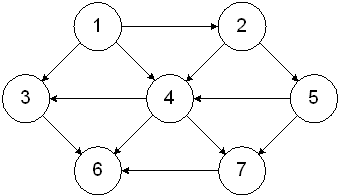
\includegraphics[width=0.4\textwidth]{graph-directed}
        \caption{Ejemplo de \emph{Grafo Dirigido No Ponderado}. (Extraído de \cite{freedman2010graphs})}
        \label{img:directed_graph_example}
      \end{figure}

      \paragraph{}
      A través de la modificación de la distribución de probabilidad del vector $p$ se consigue por tanto la adaptación del ranking \emph{PageRank} desde una perspectiva de localidad, lo cual se convierte en una clasificación mucho más interesante desde el punto de vista del usuario, que en el caso del grafo de la web, conoce de manera mucho más fiel las páginas web que son importantes desde su perspectiva individual.

      \paragraph{}
      Sin embargo, la personalización del ranking \emph{PageRank} conlleva distintos problemas a nivel computacional. Esto se debe a que en este caso en lugar de tener que mantener un único ranking para todo el grafo es necesario mantener un ranking para cada usuario que pretenda consultar el pagerank del grafo. Este problema no es tan grave como parede puesto que el vector de la distribución estacionaria $\pi$ posee la propiedad de linealidad, lo cual simplifica dicha problemática, reduciendo el problema a la necesidad de mantener un vector $\pi$ para cada vértice del grafo, es decir, hay que generar $n$ vectores \emph{PageRank}.

      \paragraph{}
      Ahora supongamos que un determinado usuario desea calcular su propio ranking personalizado. La tarea se reduce a realizar una media ponderada sobre los vectores $\pi_i$ escogiendo los pesos según el vector $p$ de personalización para dicho usuario. A pesar de ello, esta tarea continua siendo compleja, tanto a nivel temporal como espacial, puesto que se incrementa el coste respecto del \emph{PageRank General} en un orden de $n$.

      \paragraph{}
      Debido al tamaño de grafos como el de la web (\emph{Web Graph}), cuyo número de vértices es tan elevado que no es posible mantener un vector \emph{PageRank} para cada uno de ellos en memoria. Esta razón dificulta la tarea de calcular el ranking personalizado para un determinado usuario en tiempo de consulta. Por tanto, se ha se han propuesto distintas soluciones para este problema.

      \paragraph{}
      Una de las primeras es la descrita en \cite{haveliwala2002topic}, que se basa en el mantenimiento de \emph{16} vectores \emph{PageRank} de referidos a temas distintos entre si, que después se combinan en tiempo de consulta para generar un ranking personalizado. En \cite{kamvar2003exploiting} los autores proponen el cálculo de vectores \emph{PageRank} teniendo en cuenta la estructura de bloques que se genera entre vértices cuyo ranking es similar. Esto se lleva a cabo a partir de un algoritmo de 3 fases (búsqueda de vértices similares, cálculo del vector \emph{PageRank} para los conjuntos resultantes y, en tiempo de consulta, combinación de los mismos para obtener el ranking personalizado).

      \paragraph{}
      En \cite{jeh2003scaling} se explica una técnica que permite calcular el vector \emph{PageRank} personalizado utilizando una técnica incrementa o jerárquica basada en \emph{Programación Dinámica}, lo cual permite hacer calcular el ranking basado en la combinación de cien mil vectores en tiempo de consulta. En \cite{sarlos2006randomize} se propone una solución semejante en un espacio menor mediante la utilización del \emph{Count-Min Sketch} (Sección \ref{sec:count_min_sketch}).En el trabajo \emph{Estimating pagerank on graph streams} \cite{sarma2011estimating} \emph{Sarma y otros} proponen un algoritmo basado en la generación de paseos aleatorios para estimar el ranking \emph{PageRank} sobre las restricciones que impone el \emph{modelo en semi-streaming}.

    \section{Alternativas a PageRank}
    \label{sec:pagerank_alternativas}

      \paragraph{}
      El algoritmo \emph{PageRank} se ha convertido en la alternativa más usada para el cálculo del ránking de vértices sobre un grafo basándose únicamente en la estructura del mismo (relaciones a partir de aristas). Su popularidad se debe en gran medida tanto a su sencillez desde el punto de vista algorítmico (a pesar de que su coste computacional es elevado), como a la gran fama del motor de búsquedas \emph{Google}, que desde sus comienzos otorgaba resultados muy buenos apoyándose en la utilización de dicho ranking.

      \paragraph{}
      Sin embargo, \emph{PageRank} no es la única alternativa sobre la que se ha trabajado en el ámbito del cálculo de importancia para los vértices de grafos. En esta sección se describen brevemente distintos algoritmos cuya finalidad es semejante. Además se hablará de una extensión del \emph{PageRank} conocida como \emph{SimRank} que obtiene el grado de similitud entre los vértices del grafo desde un punto de vista estructural. En la sección \ref{sec:hits} se describe \emph{HITS}, posteriormente en la sección \ref{sec:salsa} se describe \emph{SALSA} (una mejora respecto del anterior), y finalmente, en la sección \ref{sec:simrank} se hablará de \emph{SimRank}.

      \subsection{HITS}
      \label{sec:hits}

        \paragraph{}
        El algoritmo \emph{HITS} surge en paralelo junto con \emph{PageRank}, puesto que los artículos en los que se habla de dichos algoritmos fueron publicados en \emph{1999}. \emph{HITS} fue descrito por primera vez en el trabajo \emph{Authoritative sources in a hyperlinked environment} \cite{kleinberg1999authoritative} de \emph{Kleinberg}.

        \paragraph{}
        Este algoritmo, a diferencia del \emph{PageRank}, se basa en la generación del ranking en tiempo de consulta. Para ello utiliza un sub-conjunto de vértices inicial obtenido a partir del ranking del ranking de similitud basada en texto respecto de la consulta en cuestión. A partir del sub-grafo generado por este sub-conjunto. Las iteraciones del algoritmo se basan la generación de dos puntuaciones para cada vértice. Estas puntuaciones se conocen como \emph{Autority score} y \emph{Hub score}. Las cuales se construyen como la suma de \emph{Hub scores} de los vértices que apuntan hacia el vértice para el caso del \emph{Autority score} y la suma de \emph{Autority scores} de los vértices hacia los que apunta el vértice para el \emph{Hub score}. Dichos valores son normalizados en cada iteración. Este proceso se repite hasta llegar a un determinado grado de convergencia.

        \paragraph{}
        Las diferencias respecto del \emph{PageRank} por tanto se basan en la generación del ranking en tiempo de consulta en lugar de en tiempo de indexación o estático, por tanto este ranking varía respecto de cada búsqueda. En este caso, en lugar de obtener un único ranking se obtienen dos, indicando los vértices más importantes y indicando los vértices que más importancia generan. Además, en lugar de generar el ranking sobre el grafo completo, \emph{HITS} lo lleva a cabo sobre un sub-grafo del mismo (obtenido mediante búsqueda textual tal y como se ha indicado anteriormente).

      \subsection{SALSA}
      \label{sec:salsa}

        \paragraph{}
        El algoritmo \emph{SALSA} se refiere a una combinación de \emph{PageRank} y \emph{HITS} (descrito en la anterior sección), por tanto, tiene características semejantes de ambas alternativas. La descripción del mismo fue llevada a cabo en el documento \emph{SALSA: the stochastic approach for link-structure analysis}\cite{lempel2001salsa} de \emph{Lempel y Moran}.

        \paragraph{}
        Debido a que este algoritmo consiste en una combinación de los citados previamente, a continuación se indican las semejanzas que tiene respecto de estos. \emph{SALSA} se basa en la misma idea que \emph{HITS}, en el sentido de que genera dos ranking, referidos a autoridades y generadores de autoridad (\emph{Autority} y \emph{Hub}). Además, también realiza dicho ranking en tiempo de consulta utilizando un sub-grafo generado a partir del ranking de similitud textual. La diferencia respecto de \emph{HITS} se basa en la estrategia utilizada para calcular dichos ranking. En este caso utiliza el mismo enfoque de \emph{paseos aleatorios} del \emph{PageRank} (por eso se dice que es una combinación de ambos).

        \paragraph{}
        La generación de rankings a través de paseos aleatorios le otorgo una ventaja significativa a nivel de coste computacional respecto de \emph{HITS}, además de ofrecer resultados en tiempo de consulta, lo cual le diferencia de \emph{PageRank}. En el documento \emph{WTF: The Who to Follow Service at Twitter} \cite{gupta2013wtf} los autores describen cómo la red social \emph{Twitter} ha desarrollado una variación de este algoritmo para su sistema de recomendación de usuarios a los que comenzar a seguir.

      \subsection{SimRank}
      \label{sec:simrank}

        \paragraph{}
        El algoritmo \emph{SimRank} tiene un propósito distinto respecto de los descritos anteriormente. En este caso, en lugar de tratar de conocer el grado de importancia de un determinado vértice del grafo, lo que se pretende es obtener un ranking de similitud del resto de vértices del grafo respecto de uno concreto. En el trabajo \emph{SimRank: a measure of structural-context similarity} \cite{jeh2002simrank} de \emph{Jeh y Widom} se describe de manera el completa el modo de funcionamiento del algoritmo, así como la demostración acerca de la corrección del mismo. A continuación se realiza una breve descripción acerca de dicho modo de funcionamiento.

        \paragraph{}
        Al igual que el \emph{PageRank}, en este caso el algoritmo también se basa en el cálculo iterativo del ranking hasta llegar a un determinado índice de convergencia. La primera iteración se basa en el cálculo de un \emph{PageRank Personalizado} desde el vértice sobre el cual se pretende basar la comparación. Tras esta inicialización, el resto del algoritmo se basa en la repetición de la ecuación \eqref{eq:simrank_iteration} hasta llegar a un índice de convergencia.

        \begin{equation}
        \label{eq:simrank_iteration}
          Sim^{(k)}_{u_1}({u_2}) =
          \begin{cases}
            (1-c) * \frac{\sum_{\{(u_1,v_1),(u_2,v_2)\} \in E} Sim^{(k-1)}_{v_1}({v_2})}{d^-({u_1})*d^-({u_2})}, & \text{if} \ u_1 \neq u_2 \\
            1, & \text{if} \ u_1 = u_2
          \end{cases}
        \end{equation}

        \paragraph{}
        La ecuación \eqref{eq:simrank_iteration} calcula por tanto el grado de similitud del vértice $u_2$ respecto del vértice $u_1$ en la iteración $k$, lo cual se puede denotar como $Sim^{(k)}_{u_1}({u_2})$. Tal y como se ha indicado anteriormente, dicho valor se incrementa conforme los vértices $u_1$ y $u_2$ se relacionan con conjuntos similares de vértices desde el punto de vista de que estos sean los mismos. Esto no debe confundirse con otros problemas como el de \emph{Matchings} (referido a encontrar subestructuras con la misma forma dentro de un grafo).

        \paragraph{}
        Existen numerosas aplicaciones prácticas para este algoritmo como sistema de recomendaciones sobre conjuntos de datos con estructura de grafo. Algunos ejemplos donde podría ser utilizado es en problemas como la generación de anuncios de sitios web en un buscador, la generación de listas de reproducción de vídeo a partir de un determinado vídeo teniendo en cuenta la navegación que los usuarios han llevado a cabo previamente entre estos, o un sistema de recomendación de compras en una tienda virtual basándose en la misma idea.

    \section{Conclusiones}
    \label{sec:pagerank_conclusions}

      \paragraph{}
      Tal y como se ha visto a lo largo del capítulo, el cálculo de importancia sobre los vértices grafos es una tarea compleja, cuya dificultad se incrementa en gran medida cuando el tamaño del grafo es de tamaño masivo, lo cual dificulta la tarea de contenerlo de manera completa en memoria. Sin embargo, en este capítulo no se han discutido soluciones para dicho problema, sino que se ha realizado un estudio acerca del algoritmo \emph{PageRank}, el cual goza de gran popularidad gracias a motor de búsquedas \emph{Google}.

      \paragraph{}
      A partir de la descripción de este algoritmo se ha podido comprender la perspectiva algebraica para la resolución de un problema sobre grafos, que puede entenderse como uno problema de matrices. Además, se ha ilustrado la cercanía de este ranking respecto de las \emph{Cadenas de Markov} y los paseos aleatorios, que convergen hacia la \emph{distribución estacionaria}. Después se ha indicado cómo calcularla a partir de distintas estrategias (\emph{Algebraica}, \emph{Iterativa} o \emph{basada en paseos aleatorios})

      \paragraph{}
      Posteriormente también se habló del \emph{PageRank Personalizado} y la problemática referida a la cantidad de rankings que sería necesario mantener para llevar a cabo una solución exacta para dicho problema. Por último se ha hablado de estrategias similares para el ranking de vértices así como el algoritmo \emph{SimRank}, que indica el grado de similitud de vértices respecto de un determinado vértice.

      \paragraph{}
      Gracias a este algoritmo se puede obtener un indicador acerca de la importancia de los vértices de un determinado grafo, lo cual es una tarea interesante y aplicable sobre un gran conjunto de ámbitos para los cuales el problema puede ser modelizado como una red. La observación acerca de la importancia de los vértices desde el punto de vista estructural es un factor interesante que puede mejorar la toma de decisiones en un gran número de casos.

\end{document}
